\documentclass{article}
\usepackage{graphicx} % Required for inserting images
\usepackage{url}
\usepackage{here}
\usepackage{amsmath,amssymb}
\usepackage{pdfpages}
%\usepackage{graphicx}
\usepackage{graphicx}   % ← ここが肝心
\usepackage{geometry}   % geometry も合わせておくと安全
\geometry{margin=1in}
\usepackage{amsthm} % For proof environment
\usepackage{physics}

\usepackage{tikz}            % TikZ 本体
\usepackage{pgfplots}        % 関数プロット用
\pgfplotsset{compat=1.18}    % バージョン依存の警告防止

\newcommand{\B}[1]{\mathbf{#1}}
\newcommand{\T}[1]{\tilde{#1}}
\newcommand{\V}{\hat{V}}
\newcommand{\cov}{\widehat{cov}}
\newcommand{\argmax}{\mathop{\rm arg~max}\limits}
\newcommand{\argmin}{\mathop{\rm arg~min}\limits}

\title{HW2}
\author{Kosuke IGARASHI 29-246004}
\date{June 2025}

\begin{document}

\maketitle

\section{Exercise 22.1}

The model is
\[
Y = X'\theta + e,
\]
where $e$ is independent of $X$ and density function $f(e)$ is known and continuously differentiable .

\bigskip

\subsection*{(a)}
Because $Y = X' \theta + e$, so $e = Y - X' \theta$.\\
$e$ is independent of $X$ and has density $f(e)$, the conditional density of $Y$ given $X = x$ is:
\[
f_{Y|X}(y|x) = f(y - x'\theta).
\]
\bigskip

\subsection*{(b)}
The log-likelihood for a single observation is $\ell(\theta) = \log f(y - x'\theta)$.\\
Let me define the M-estimator objective function as $\rho(Y,X,\theta) = -\log f(Y - X'\theta)$.
The score function is:
\[
\psi(Y,X,\theta) = \frac{\partial}{\partial \theta} \log f(Y - X'\theta).
\]
By the chain rule, we have:
\[
\psi(Y,X,\theta) = -\frac{f'(Y - X'\theta)}{f(Y - X'\theta)} \cdot (-X) = -X \cdot \frac{f'(Y - X'\theta)}{f(Y - X'\theta)}.
\]

\bigskip

\subsection*{(c)}
We assume some regularity conditions for the m-estimator.\\

The asymptotic covariance matrix of the M-estimator is
\begin{align*}
    \Sigma &= H^{-1} S H^{-1}\\
    \text{where } H = E\left[ -\frac{\partial}{\partial \theta'} \psi(Y,X,\theta_0) \right] \text{, } S = E\left[ \psi(Y,X,\theta_0) \psi(Y,X,\theta_0)' \right].
\end{align*}

To compute $H$, we differentiate $\psi(Y,X,\theta) = -X \cdot \frac{f'(Y - X'\theta)}{f(Y - X'\theta)},$ with respect to $\theta'$,
\begin{align*}
    -\frac{\partial}{\partial \theta'} \psi(Y,X,\theta) = -X X' \cdot \left[ \frac{f''(Y - X'\theta) f(Y - X'\theta) - (f'(Y - X'\theta))^2 }{ f(Y - X'\theta)^2 } \right]    
\end{align*}

We evaluate this at the true parameter $\theta_0$ and take the expectation to compute $H$. Thus, we have
\[
H=E\left[-X X' \cdot \left[ \frac{f''(Y - X'\theta_0) f(Y - X'\theta_0) - (f'(Y - X'\theta_0))^2 }{ f(Y - X'\theta_0)^2 } \right] \right].
\]

Then, 
\[
S = E\left[ X X' \cdot \left( \frac{f'(Y - X'\theta_0)}{f(Y - X'\theta_0)} \right)^2 \right].
\]

Finally, the asymptotic covariance matrix is:
\begin{align*}
    \Sigma
    &= H^{-1} S H^{-1},
\end{align*}
which can be explicitly evaluated depending on the known density $f$ and the distribution of $X$.

\section{Exercise 22.3}

\begin{figure}[htbp]
  \centering
  %------------------------- TikZ picture --------------------------
  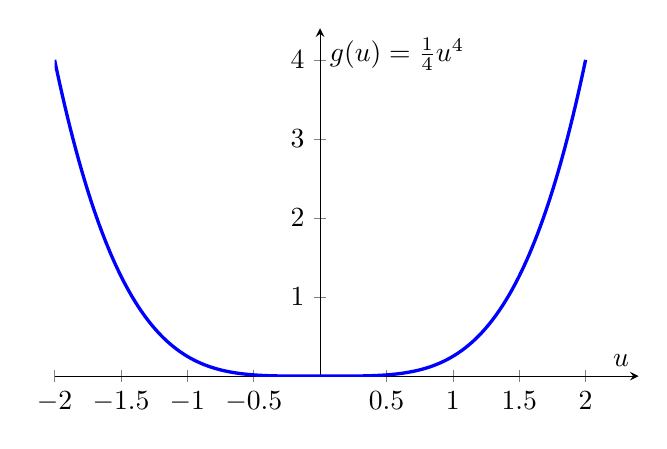
\begin{tikzpicture}
    \begin{axis}[
      % --- 軸の設定 ---
      axis lines = middle,
      xlabel     = {$u$},
      ylabel     = {$g(u)=\tfrac14 u^4$},
      domain = -2:2,            % x 範囲
      samples = 200,            % 描画点数
      ymin = 0,                 % y の下限
      enlargelimits = upper,    % 上側に少し余白
      width = 9cm, height = 6cm % 絵のサイズ(任意)
    ]
      \addplot[very thick, blue] {0.25*x^4};
    \end{axis}
  \end{tikzpicture}
  %----------------------------------------------------------------
  \caption{Graph of $g(u)=\tfrac14 u^{4}$ on $[-2,2]$}
  \label{fig:g_quarter_u4}
\end{figure}

\begin{itemize}
    \item[(a)]
    \textbf{(i) Continuity.}  
    Fix $u_0\in\mathbb R$ and $\varepsilon>0$.  Choose
    \[
    \delta \;=\;\min\!\left\{1,\frac{\varepsilon}{\bigl(1+|u_0|\bigr)^{3}}\right\}.
    \]
    Whenever $\lvert u-u_0\rvert<\delta$, write $u=u_0+h$ with $\lvert h\rvert<\delta\le1$.  A straightforward expansion gives
    \[
    \bigl|g(u)-g(u_0)\bigr|
       = \frac14\bigl|(u_0+h)^4-u_0^{4}\bigr|
       = \frac14\bigl|4u_0^{3}h+6u_0^{2}h^{2}+4u_0h^{3}+h^{4}\bigr|.
    \]
    Using $\lvert h\rvert<1$ and $\lvert h\rvert<\delta$, 
    \begin{align*}
        \bigl|g(u)-g(u_0)\bigr|
      &\le |u_0|^{3}\lvert h\rvert
         +\tfrac32 |u_0|^{2}|h|^{2}
         +|u_0| |h|^{3}
         +\tfrac14 |h|^{4}\\
         &<(|u_0|^3+\tfrac32 |u_0|^{2}+|u_0|+\tfrac14)|h|\\
      &< \bigl(1+|u_0|\bigr)^{3}\lvert h\rvert
      <\varepsilon.
    \end{align*}

    Hence $g$ is continuous at $u_0$; since $u_0$ was arbitrary, $g$ is continuous on $\mathbb R$.
    
    \medskip\noindent
    \textbf{(ii) Differentiability.}  
    For $u_0\in\mathbb R$, consider the difference quotient
    \[
    \frac{g(u_0+h)-g(u_0)}{h}
      =\frac{(u_0+h)^{4}-u_0^{4}}{4h}
      =u_0^{3}+\frac{3}{2}u_0^{2}h+u_0h^{2}+\frac14 h^{3}.
    \]
    Taking the limit $h\to0$,
    \[
    \lim_{h\to0}\frac{g(u_0+h)-g(u_0)}{h}=u_0^{3},
    \]
    so the derivative exists and equals $u_0^{3}$.
    
    \medskip\noindent
    \textbf{(iii) Continuity of the derivative.}  
    For $u_0\in\mathbb R$, consider the difference quotient
    \[
    \frac{g'(u_0+h)-g'(u_0)}{h}
      =\frac{(u_0+h)^{3}-u_0^{3}}{h}
      =3u_0^{2}+3u_0h^{}+ h^{2}.
    \]
    Taking the limit $h\to0$,
    \[
    \lim_{h\to0}\frac{g'(u_0+h)-g'(u_0)}{h}=3u_0^{2},
    \]
    so the second derivative exists and equals $3u_0^{2}$.

    \item[(b)]
    \[
    \rho(Y,X,\theta)=\tfrac14 \bigl(Y-X'\theta\bigr)^{4},
    \ 
    \psi(Y,X,\theta)= \frac{\partial \rho(Y,X,\theta)}{\partial\theta}=-X\bigl(Y-X'\theta\bigr)^3 .
    \]

    \item[(c)]
    The asymptotic covariance matrix of the m-estimator is
    \begin{align*}
        \Sigma = H^{-1} S [H^{-1}]\\
        \text{where } H = E\left[ -\frac{\partial}{\partial \theta'} \psi(Y,X,\theta_0) \right] \text{, } S = E\left[ \psi(Y,X,\theta_0) \psi(Y,X,\theta_0)' \right]
    \end{align*}
    
    To compute $H$, we differentiate $\psi(Y,X,\theta)$ with respect to $\theta'$
    \begin{align*}
         -\frac{\partial}{\partial \theta'} \psi(Y,X,\theta) = -3X X' (Y-X'\theta)^2
    \end{align*}

    We evaluate this at the true parameter $\theta_0$ and take the expectation to compute $H$.
    
    we have S from (b), $S = E\left[ X X' (Y-X'\theta_0)^6 \right]$.
    
    Finally, the asymptotic covariance matrix is
    \[
    \frac{1}{9}\bigl(E[X X' (Y-X'\theta_0)^2])^{-1}
          \; E\left[ X X' (Y-X'\theta_0)^6 \right]\;
          \bigl(E[X X' (Y-X'\theta_0)^2])^{-1}.
    \]
\end{itemize}


\section{Exercise 23.8}
\textbf{Attached at the end of this document.}

\section{Exercise 24.6}

\begin{align*}
    \mathbb{E}[\psi_\tau(e)|X] &= \mathbb{E}[\tau - \mathbb{I} (e<0)|X] \\
    &= \tau - \mathbb{P}[Y < q_\tau(X)|X]\\
    &= \tau - \mathbb{P}[Y \leq q_\tau(X)|X] \quad(\because \mathbb{P}[Y = q_\tau(X)] = 0)\\
    &= \tau - \tau \quad(\because \text{Definition of conditional quantile})\\
    &= 0
\end{align*}

\section{Exercise 24.13}
\textbf{Attached at the end of this document.}
 
\section{Exercise 13.4}
Assume $W$ is a positive definite symmetric matrix.

\begin{itemize}
    \item[(a) ]
    \begin{align*}
        V_0 &= (Q'\Omega^{-1}Q)^{-1}Q'\Omega^{-1}\Omega\Omega^{-1}Q(Q'\Omega^{-1}Q)^{-1} \\
        &= (Q'\Omega^{-1}Q)^{-1}Q'\Omega^{-1}Q(Q'\Omega^{-1}Q)^{-1} \\
        & = (Q'\Omega^{-1}Q)^{-1}.
    \end{align*}

    \item[(b) ]
    $A = WQ(Q'WQ)^{-1}$ and $B = \Omega^{-1}Q(Q'\Omega^{-1}Q)^{-1}$ yield $V = A'\Omega A, V_0 = B'\Omega B$.

    \item[(c) ]
    \begin{align*}
        B'\Omega A &= (Q'\Omega^{-1}Q)^{-1}Q'\Omega^{-1}WQ(Q'WQ)^{-1} \\
        &= (Q'\Omega^{-1}Q)^{-1}\\
        &= B'\Omega B.
    \end{align*}
    Therefore, $B'\Omega(A - B) = 0$.

    \item[(d) ]
    We have
    \begin{align*}
        V &= A'\Omega A \\ 
        &= (B + A - B)'\Omega(B + A - B) \\
        &= B'\Omega B + (A - B)'\Omega(A - B) \\
        &= V_0 + (A - B)'\Omega(A - B) \\
        &\geq V_0 
    \end{align*}
\end{itemize}

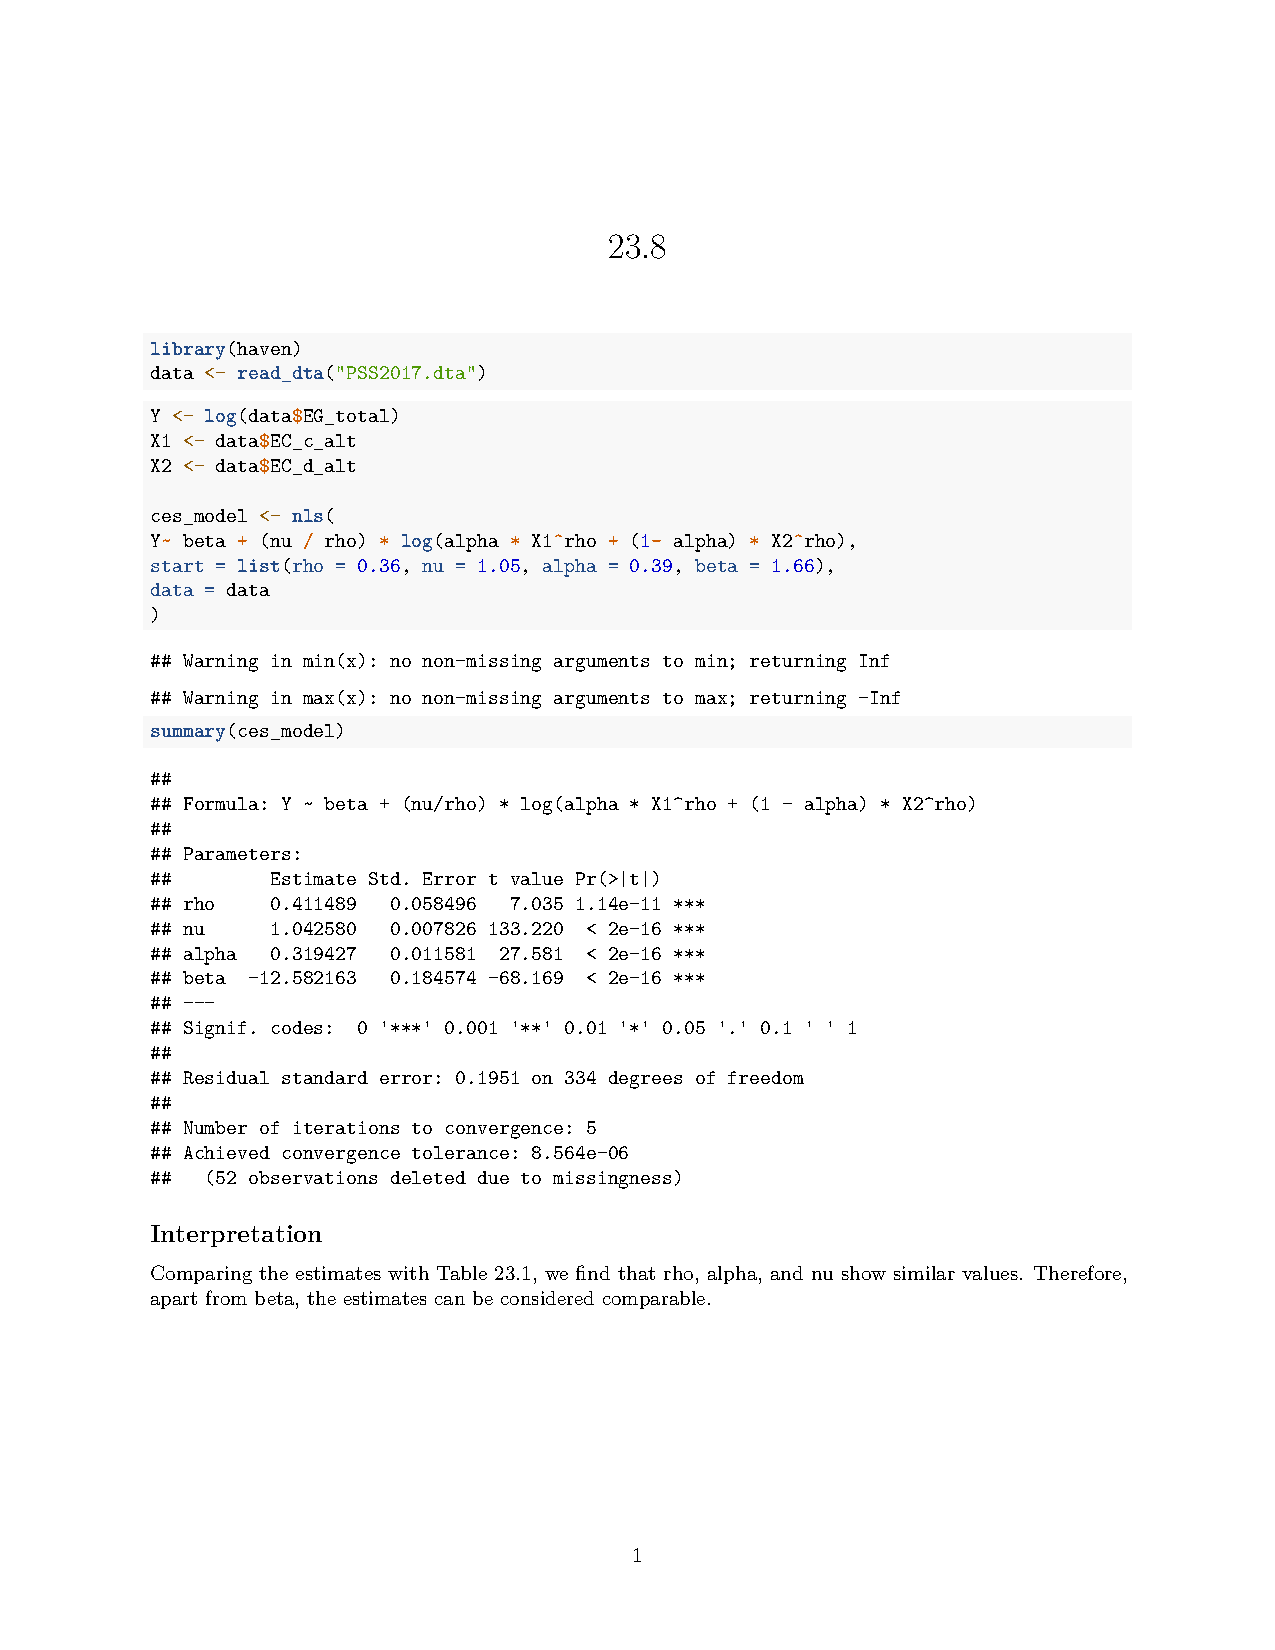
\includepdf[
  pages = - ,        % すべてのページ。1-3 のように範囲指定も可
  pagecommand = {}   % 既存のヘッダ/フッタを消して真っ白に
]{23.8.pdf}

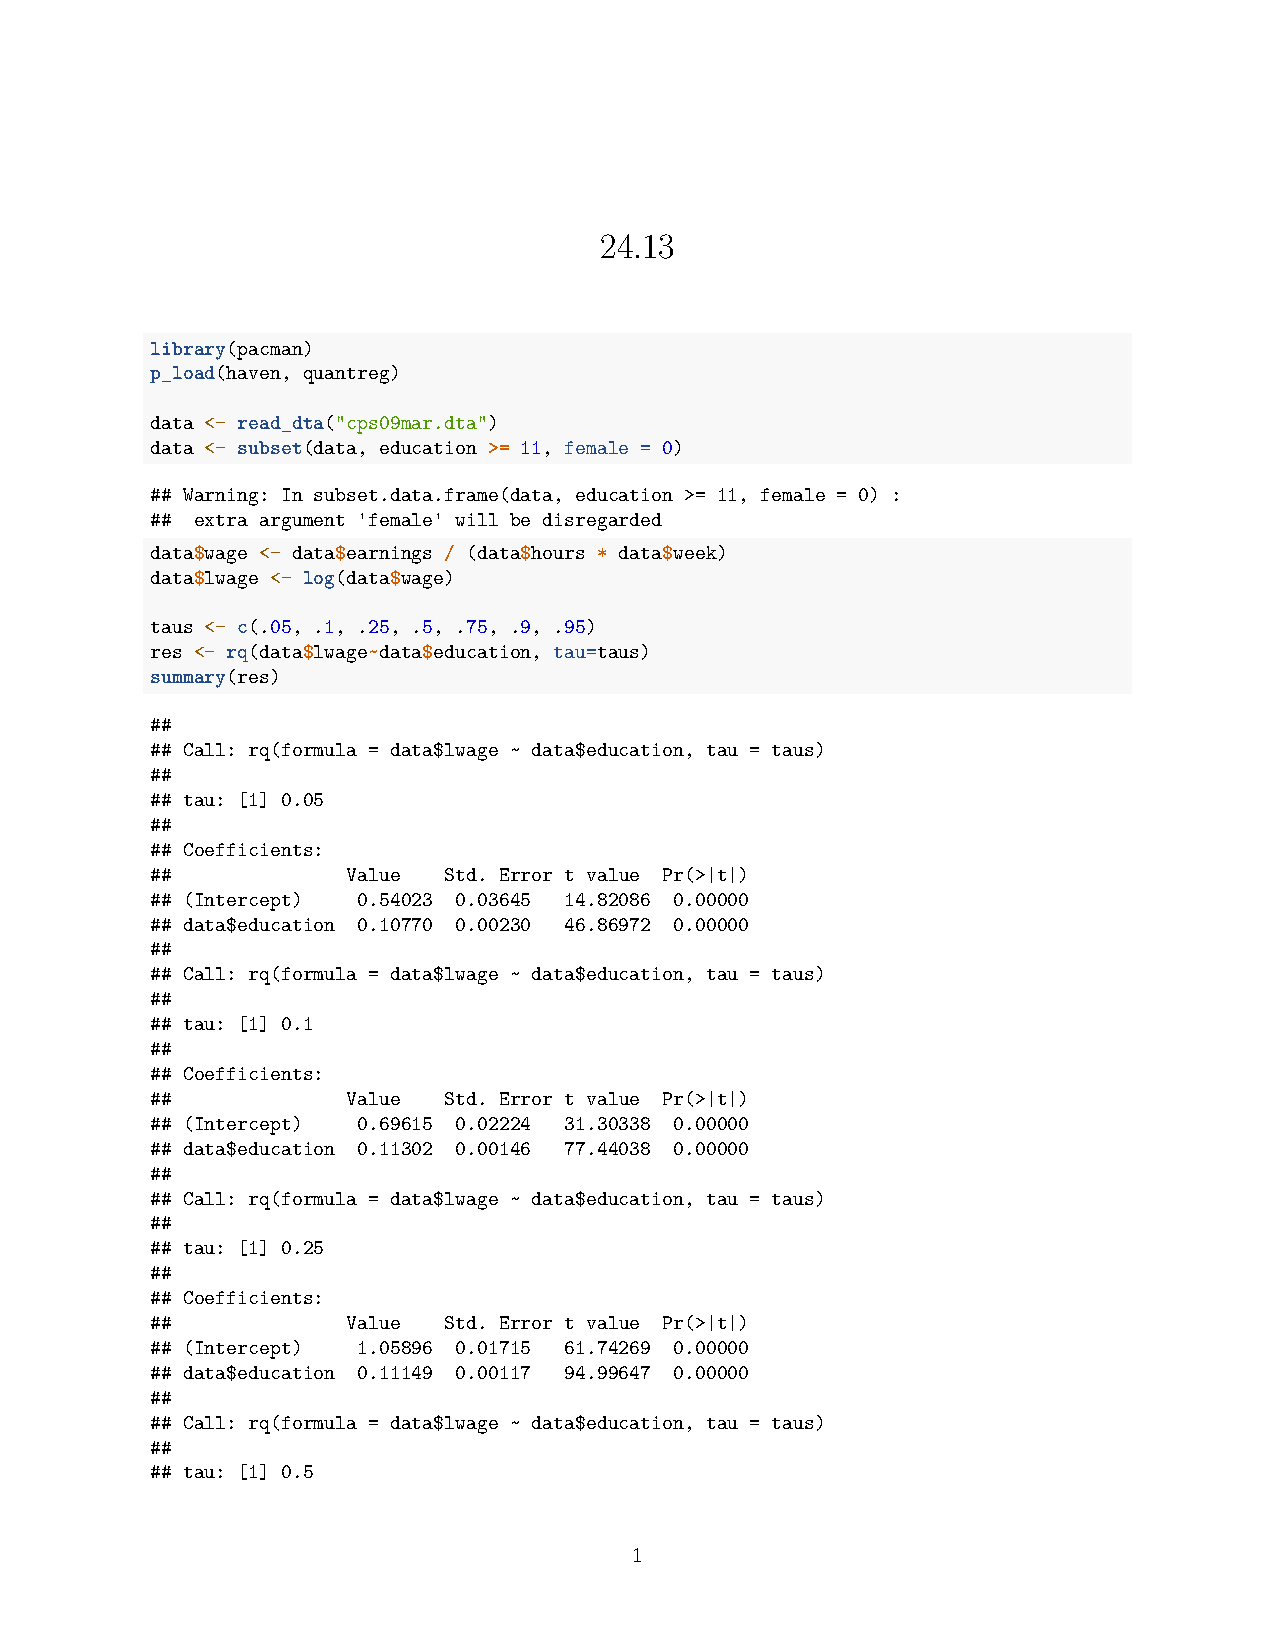
\includepdf[
  pages = - ,        % すべてのページ。1-3 のように範囲指定も可
  pagecommand = {}   % 既存のヘッダ/フッタを消して真っ白に
]{24.13.pdf}

\end{document}
